% --- Data parallelism ---
\begin{frame}{Data Parallelism: Replicate the Model, Split the Batch}
  \begin{columns}[T,onlytextwidth]
    \column{0.55\textwidth}
      \begin{itemize}\footnotesize\itemsep0.35em
        \item[\textcolor{red}{$\blacktriangleright$}] Give every one of $d$ ranks a \textbf{complete copy} of the model and $1/d$ of the global batch. Each rank runs its own forward and backward pass with no communication at all.
        \item[\textcolor{red}{$\blacktriangleright$}] Correctness rests on one fact: the gradient of a sum is the sum of the gradients. If rank $r$ holds micro-batch $\mathcal{B}_r$, then
          \[
            \nabla_\theta \mathcal{L}\!\left(\textstyle\bigcup_r \mathcal{B}_r\right)
            \;=\; \frac{1}{d}\sum_{r=1}^{d} \nabla_\theta \mathcal{L}(\mathcal{B}_r).
          \]
        \item[\textcolor{red}{$\blacktriangleright$}] So the \textbf{only} synchronisation needed is one \textbf{all-reduce} over the gradient buffer at the end of the backward pass. After it, every rank holds the identical averaged gradient and takes an identical optimizer step, so the replicas never diverge.
        \item[\textcolor{red}{$\blacktriangleright$}] This is why data parallelism is the default: it is one collective per step, it needs no change to the model code, and it scales throughput almost linearly --- \emph{as long as the model fits on one device}.
      \end{itemize}
    \column{0.43\textwidth}
      \centering
      \vspace{0.9em}
      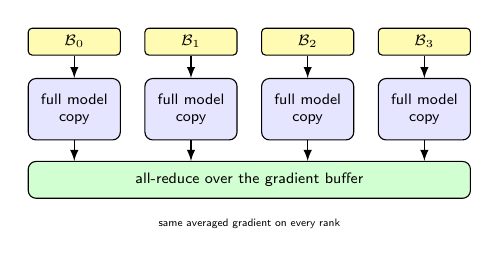
\begin{tikzpicture}[font=\sffamily\scriptsize, >=latex, scale=0.78,
          every node/.style={transform shape},
          gpu/.style={draw, rounded corners=0.1cm, fill=blue!10, minimum width=1.5cm, minimum height=1.0cm, align=center},
          bat/.style={draw, fill=yellow!30, minimum width=1.5cm, minimum height=0.42cm, rounded corners=0.05cm}]
        \foreach \i/\x in {0/0, 1/1.9, 2/3.8, 3/5.7} {
          \node[bat] (b\i) at (\x,2.35) {$\mathcal{B}_{\i}$};
          \node[gpu] (g\i) at (\x,1.25) {full model\\copy};
          \draw[->] (b\i.south) -- (g\i.north);
        }
        \node[draw, fill=green!18, rounded corners=0.1cm, minimum width=7.2cm, minimum height=0.6cm] (ar) at (2.85,0.1)
          {all-reduce over the gradient buffer};
        \foreach \i in {0,...,3} {\draw[->] (g\i.south) -- (g\i.south |- ar.north);}
        \node[font=\sffamily\tiny] at (2.85,-0.62) {same averaged gradient on every rank};
      \end{tikzpicture}
  \end{columns}
\end{frame}

\begin{frame}{What an All-Reduce Actually Costs}
  \centering
  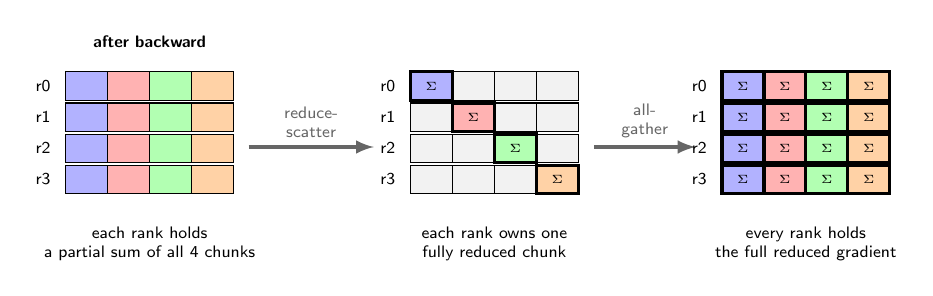
\begin{tikzpicture}[font=\sffamily\scriptsize, >=latex, scale=0.86,
      every node/.style={transform shape},
      cell/.style={draw, minimum width=0.62cm, minimum height=0.42cm},
      lbl/.style={font=\sffamily\scriptsize}]
    % Stage 1: local gradients
    \node[lbl, anchor=south] at (1.24,1.55) {\textbf{after backward}};
    \foreach \rr in {0,...,3} {
      \node[lbl, anchor=east] at (-0.1,{1.1-0.46*\rr}) {r\rr};
      \foreach \cc/\colr in {0/blue!30, 1/red!30, 2/green!30, 3/orange!35} {
        \node[cell, fill=\colr] at ({0.31+0.62*\cc},{1.1-0.46*\rr}) {};
      }
    }
    \node[lbl, anchor=north, align=center] at (1.24,-0.85) {each rank holds\\a partial sum of all 4 chunks};
    \draw[->, very thick, black!60] (2.70,0.2) -- (4.55,0.2) node[midway, above, lbl, align=center] {reduce-\\scatter};
    % Stage 2: reduce-scatter result. Only the diagonal cell is owned by that rank.
    \foreach \rr/\colr in {0/blue!30, 1/red!30, 2/green!30, 3/orange!35} {
      \node[lbl, anchor=east] at (4.99,{1.1-0.46*\rr}) {r\rr};
      \foreach \cc in {0,...,3} {
        \node[cell, fill=black!5] at ({5.40+0.62*\cc},{1.1-0.46*\rr}) {};
      }
      \node[cell, fill=\colr, very thick] at ({5.40+0.62*\rr},{1.1-0.46*\rr}) {\tiny$\Sigma$};
    }
    \node[lbl, anchor=north, align=center] at (6.33,-0.85) {each rank owns one\\fully reduced chunk};
    \draw[->, very thick, black!60] (7.80,0.2) -- (9.30,0.2) node[midway, above, lbl, align=center] {all-\\gather};
    % Stage 3: all-gather result
    \foreach \rr in {0,...,3} {
      \node[lbl, anchor=east] at (9.59,{1.1-0.46*\rr}) {r\rr};
      \foreach \cc/\colr in {0/blue!30, 1/red!30, 2/green!30, 3/orange!35} {
        \node[cell, fill=\colr, very thick] at ({10.00+0.62*\cc},{1.1-0.46*\rr}) {\tiny$\Sigma$};
      }
    }
    \node[lbl, anchor=north, align=center] at (10.93,-0.85) {every rank holds\\the full reduced gradient};
  \end{tikzpicture}
  \vspace{0.4em}
  \begin{itemize}\footnotesize\itemsep0.2em
    \item[\textcolor{red}{$\blacktriangleright$}] A ring all-reduce is a \textbf{reduce-scatter} followed by an \textbf{all-gather}. Each phase moves $\frac{d-1}{d}\Psi$ elements per rank, so the round trip moves $2\frac{d-1}{d}\Psi \approx 2\Psi$ elements --- \textbf{independent of the number of ranks}.
    \item[\textcolor{red}{$\blacktriangleright$}] In \texttt{bf16} that is $4\Psi$ \emph{bytes} per rank per step: $28$\,GB for a 7B model. Tens of milliseconds inside an NVLink domain; hundreds of milliseconds over a single 400\,Gb/s InfiniBand port. It must be hidden, not merely tolerated.
  \end{itemize}
  \vspace{0.1em}
  {\scriptsize Volume analysis: Rajbhandari et al., \href{https://arxiv.org/abs/1910.02054v3}{arXiv:1910.02054v3}, section \emph{Communication Analysis of ZeRO-DP}.}
\end{frame}

\begin{frame}[allowframebreaks]{Hiding the Communication: Gradient Bucketing}
  \begin{itemize}\itemsep0.4em
    \item[\textcolor{red}{$\blacktriangleright$}] The naive implementation waits for the whole backward pass, then all-reduces one enormous buffer. The GPU sits idle for the entire collective.
    \item[\textcolor{red}{$\blacktriangleright$}] \textbf{PyTorch DDP} instead groups parameters into \textbf{buckets} (25\,MB by default) in reverse registration order. As soon as every gradient in a bucket is ready, that bucket's all-reduce is launched on a side stream while the backward pass continues through earlier layers.
    \item[\textcolor{red}{$\blacktriangleright$}] Because the backward pass produces gradients \emph{last layer first}, and the last layers are exactly the ones DDP buckets first, most of the communication overlaps with useful compute.
    \item[\textcolor{red}{$\blacktriangleright$}] Two knobs matter in practice:
      \begin{itemize}\itemsep0.15em\footnotesize
        \item \textbf{Bucket size:} too small and you pay per-collective latency; too large and there is nothing left to overlap with. NCCL needs large messages to reach peak bandwidth.
        \item \textbf{\texttt{no\_sync()}:} skip the all-reduce entirely on gradient-accumulation micro-batches.
      \end{itemize}
    \item[\textcolor{red}{$\blacktriangleright$}] With these in place, Li et al.\ report \textbf{near-linear scalability to 256 GPUs} for DDP.
    \item[\textcolor{red}{$\blacktriangleright$}] A practical corollary: \textbf{never build a DP job out of \texttt{DataParallel}} (single-process, multi-thread, scatters and gathers every step). Use \texttt{DistributedDataParallel} with one process per GPU.
  \end{itemize}
  \vspace{0.1em}
  {\scriptsize Li et al., ``PyTorch Distributed: Experiences on Accelerating Data Parallel Training,'' VLDB 2020. \href{https://arxiv.org/abs/2006.15704v1}{arXiv:2006.15704v1}}
\end{frame}

\begin{frame}[allowframebreaks]{Scaling Efficiency: When Data Parallelism Stops Paying}
  \begin{itemize}\itemsep0.4em
    \item[\textcolor{red}{$\blacktriangleright$}] Per step, the compute per rank scales with the \textbf{micro-batch} $b$, but the communication is a fixed $\approx 4\Psi$ bytes regardless of $b$. The ratio that decides your efficiency is therefore
      \[
        \frac{\text{communication}}{\text{computation}} \;\propto\; \frac{\Psi}{b \cdot s \cdot \Psi} \;=\; \frac{1}{b \cdot s}.
      \]
    \item[\textcolor{red}{$\blacktriangleright$}] Read off the three failure modes:
      \begin{itemize}\itemsep0.15em\footnotesize
        \item \textbf{Small per-device batch} (because activations do not fit) $\Rightarrow$ communication dominates. This is why activation memory and communication efficiency are the same problem.
        \item \textbf{Slow interconnect} $\Rightarrow$ the same volume takes longer. Ethernet-connected nodes fall off the linear curve far earlier than InfiniBand ones.
        \item \textbf{Too many ranks} $\Rightarrow$ the global batch grows past the point where extra examples still improve the gradient.
      \end{itemize}
    \item[\textcolor{red}{$\blacktriangleright$}] The last point is not a systems problem but a statistics one. McCandlish et al.\ formalise it with the \textbf{gradient noise scale}: beyond a \emph{critical batch size}, doubling the batch stops halving the number of steps to a given loss, so extra GPUs buy wall-clock time at a worsening compute cost.
  \end{itemize}
  \vspace{0.1em}
  {\scriptsize McCandlish, Kaplan, Amodei et al., ``An Empirical Model of Large-Batch Training,'' \href{https://arxiv.org/abs/1812.06162v1}{arXiv:1812.06162v1}.}
\end{frame}

\begin{frame}[allowframebreaks]{Large Batches Change the Optimizer}
  \begin{itemize}\itemsep0.4em
    \item[\textcolor{red}{$\blacktriangleright$}] Adding data-parallel ranks multiplies the global batch. If you leave the learning rate alone, you take the same-sized steps on a less noisy gradient and converge more slowly per epoch.
    \item[\textcolor{red}{$\blacktriangleright$}] \textbf{Linear scaling rule} (Goyal et al.): when the minibatch is multiplied by $k$, multiply the learning rate by $k$. This let them train ResNet-50 with a batch of \textbf{8192 on 256 GPUs in one hour} with no accuracy loss.
    \item[\textcolor{red}{$\blacktriangleright$}] It only works with a \textbf{gradual warmup}: the rule is derived from an approximation that fails in the first few epochs, when weights change fastest. Ramp the learning rate from small to target over a few hundred to a few thousand steps.
    \item[\textcolor{red}{$\blacktriangleright$}] At extreme batch sizes even that breaks down. \textbf{LARS} and then \textbf{LAMB} rescale the update per layer by the ratio of weight norm to update norm; LAMB trained BERT at batch \textbf{32{,}868}, cutting training from 3 days to \textbf{76 minutes}.
    \item[\textcolor{red}{$\blacktriangleright$}] For LLM pre-training the modern practice is a \textbf{batch-size warmup} as well: start with a smaller global batch and grow it as the gradient noise scale rises during training.
  \end{itemize}
  \vspace{0.1em}
  {\scriptsize Goyal et al., \href{https://arxiv.org/abs/1706.02677v2}{arXiv:1706.02677v2}; You et al., ``Large Batch Optimization for Deep Learning: Training BERT in 76 minutes,'' ICLR 2020, \href{https://arxiv.org/abs/1904.00962v5}{arXiv:1904.00962v5}.}
\end{frame}

\begin{frame}{The Wall Data Parallelism Cannot Climb}
  \begin{itemize}\itemsep0.5em
    \item[\textcolor{red}{$\blacktriangleright$}] Data parallelism gives you \textbf{throughput}, and nothing else. Every rank still stores the full $16\Psi$ bytes of model states.
    \item[\textcolor{red}{$\blacktriangleright$}] Adding GPUs therefore does not help you fit a bigger model at all. On an 80\,GB card, $80\,\text{GB} / 16\,\text{bytes} = 5\times10^{9}$ parameters exactly exhausts memory with \emph{zero} activations; allowing for activations, buffers, and fragmentation the practical ceiling is around \textbf{2--3B parameters}. Rajbhandari et al.\ report the analogous limit as \textbf{1.4B} parameters on 32\,GB cards.
    \item[\textcolor{red}{$\blacktriangleright$}] Worse, the replication is \emph{pure waste}: $d$ ranks store $d$ identical copies of the optimizer states, and each rank only ever needs $1/d$ of them at the moment of the optimizer step.
    \item[\textcolor{red}{$\blacktriangleright$}] That observation --- \emph{the redundancy is unnecessary} --- is the whole content of the next section.
  \end{itemize}
\end{frame}
